\documentclass[aspectratio=169]{beamer}
\setbeamertemplate{navigation symbols}{}
\usepackage{color, amsmath, comment, subfigure}
\usepackage{url}

\usepackage{hyperref}
\hypersetup{
    colorlinks=true,
    linkcolor=blue,
    filecolor=magenta,      
    urlcolor=cyan,
}

%%%%%%%%%%%%%%%%%%%%%%%%%%
\title[]{Pre-read for Tuesday Sept 22:\\Armed conflict, part 1}
\author[]{Matthew J. Salganik}
\institute[]{}
\date[]{COS 597E/SOC 555 Limits to prediction\\Fall 2020, Princeton University}

\begin{document}
%%%%%%%%%%%%%%%%%%%%%%%%%%%
\frame{\titlepage}
%%%%%%%%%%%%%%%%%%%%%%%%%%%
\begin{frame}
\frametitle{}

Two themes:
\begin{itemize}
\item prediction vs causation
% number of books in your house and grades
\pause
\item algorithmic modeling vs data modeling
\end{itemize}
 
\end{frame}
%%%%%%%%%%%%%%%%%%%%%%%%%%
\begin{frame}

\begin{center}
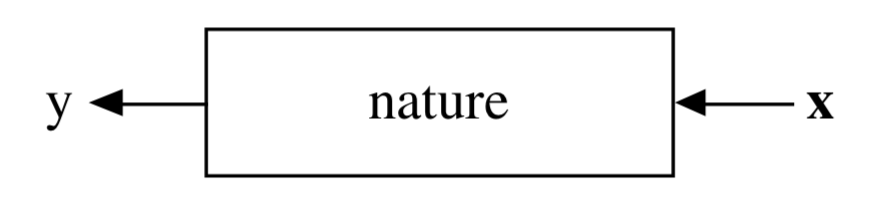
\includegraphics[width=0.30\textwidth]{figures/breiman_nature}
\end{center}

\pause

\begin{center}
\begin{tabular}{ccc}
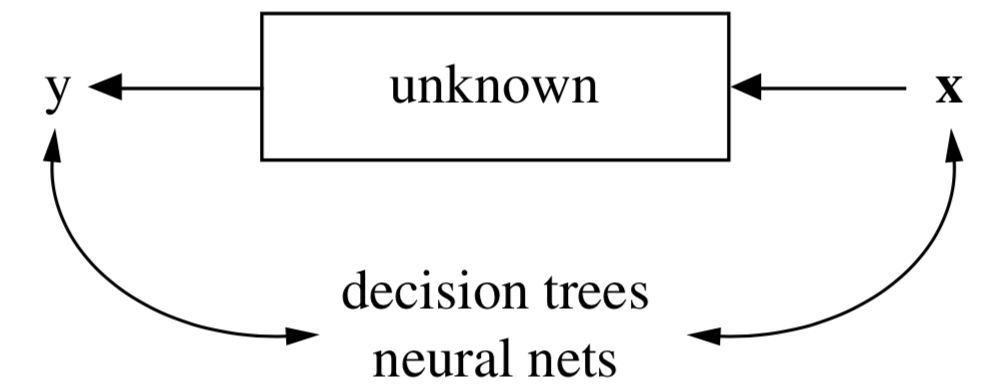
\includegraphics[width=0.30\textwidth]{figures/breiman_algorithmic_modeling} & & 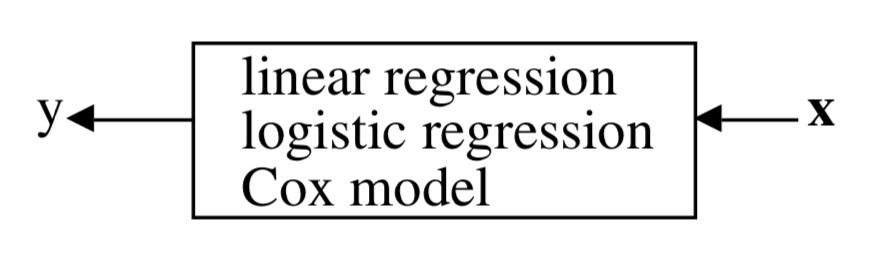
\includegraphics[width=0.30\textwidth]{figures/breiman_data_modeling} \\
\LARGE{Algorithmic modeling} &  & \LARGE{Data modeling}
\end{tabular}
\end{center}

\vfill
Breiman (2001)

\end{frame}
%%%%%%%%%%%%%%%%%%%%%%%%%
\begin{frame}
\frametitle{}

\begin{center}
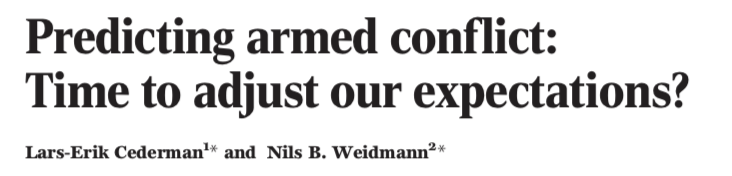
\includegraphics[width=0.9\textwidth]{figures/cederman_predicting_2017_title}
\end{center}

\end{frame}
%%%%%%%%%%%%%%%%%%%%%%%%%%%
\begin{frame}
\frametitle{}

Reading notes:
\begin{itemize}
\item Response to crazy claims about the magic of big data and machine learning
\pause
\item Lumpers vs splitters, they are splitters
\pause
\item Critical of the idea that big data and machine learning will revolutionize conflict prediction.  Why?
\end{itemize}

\end{frame}
%%%%%%%%%%%%%%%%%%%%%%%%%%%
\begin{frame}

\begin{center}
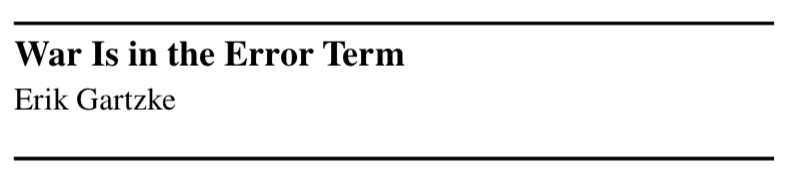
\includegraphics[width=0.9\textwidth]{figures/gartzke_war_1999_title}
\end{center}

\end{frame}
%%%%%%%%%%%%%%%%%%%%%%%%%%%
\begin{frame}

Reading notes:
\begin{itemize}
\item This paper will confusing because you are stepping into the middle a long conversation.
% Thucididies and Carl von Clauswetiz
\pause
\item ``rationalist theory'' more often called ``rational choice theory''
\pause
\item The key thing to notice in this paper is how he tries to make an model that leads to inherent unpredictability that cannot be eliminated by more research or more data or more machine learning.   Focus on the broad structure of that model.
\pause
\item Notice the he then talks about how to test the predictions from that model, not the model itself
\end{itemize}

\end{frame}
%%%%%%%%%%%%%%%%%%%%%%%%%%%
\begin{frame}

\begin{center}
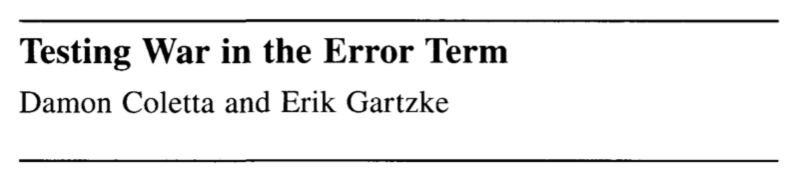
\includegraphics[width=0.9\textwidth]{figures/coletta_testing_2003_title}
\end{center}

\end{frame}
%%%%%%%%%%%%%%%%%%%%%%%%%%%
\begin{frame}

Reading notes:
\begin{itemize}
\item Beware that not all proofs are right
\pause
\item (Speculation) Many models that purport to show inherent unpredictability may prove hard to test empirically because they involve hard to measure parameters
\end{itemize}

\end{frame}
%%%%%%%%%%%%%%%%%%%%%%%%%%%
\begin{frame}

\begin{center}
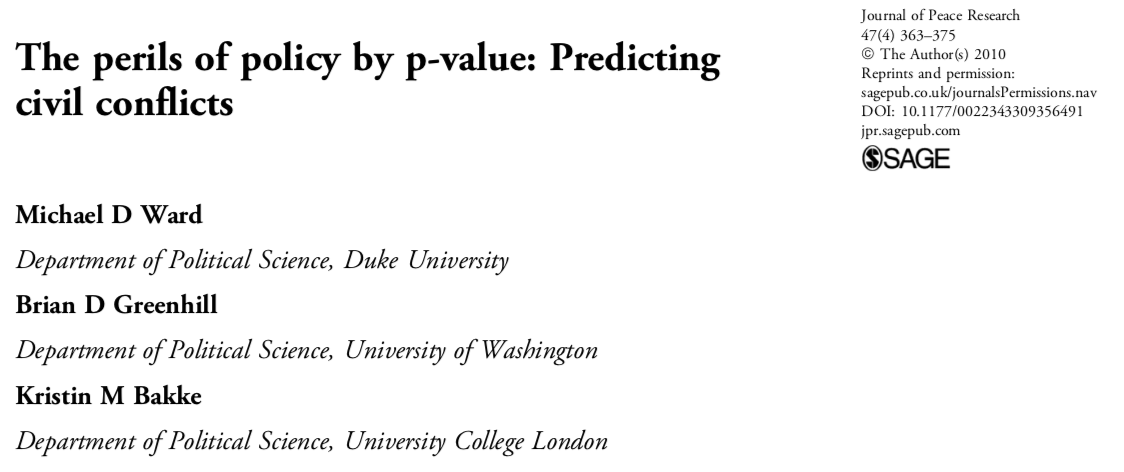
\includegraphics[height=0.7\textheight]{figures/ward_perils_2010_title}
\end{center}

\end{frame}
%%%%%%%%%%%%%%%%%%%%%%%%%%%
\begin{frame}

\begin{center}
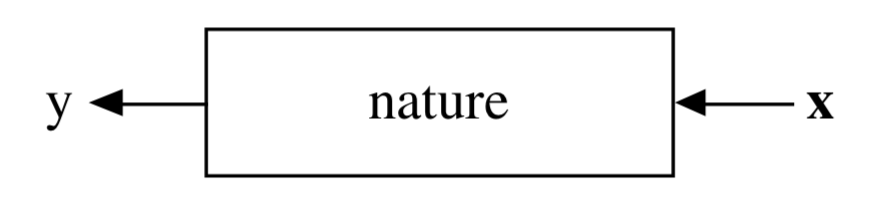
\includegraphics[width=0.30\textwidth]{figures/breiman_nature}
\end{center}

\pause

\begin{center}
\begin{tabular}{ccc}
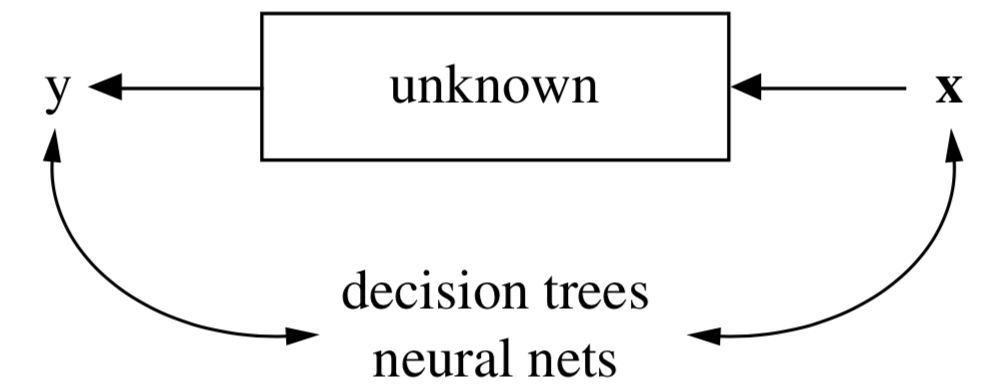
\includegraphics[width=0.30\textwidth]{figures/breiman_algorithmic_modeling} & & 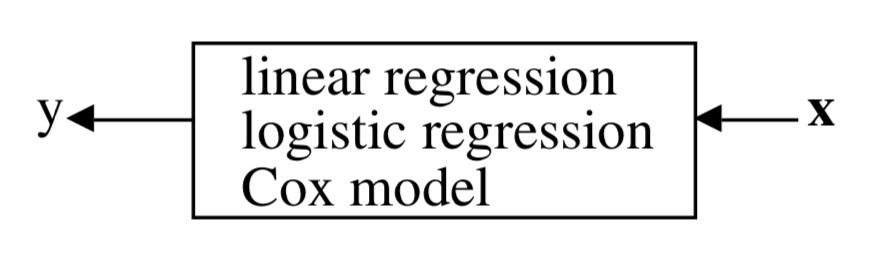
\includegraphics[width=0.30\textwidth]{figures/breiman_data_modeling} \\
\LARGE{Algorithmic modeling} &  & \LARGE{Data modeling}
\end{tabular}
\end{center}

\vfill
Breiman (2001)

\end{frame}
%%%%%%%%%%%%%%%%%%%%%%%%%
\begin{frame}

Reading notes:
\begin{itemize}
\item This is a $\hat{\beta}$ community and they are trying to bring in the $\hat{y}$
\pause
\item Research community had been searching for ways to ``understand'' civil war
\pause
\item Old idea: Civil wars caused by grievances related to ethic diversity and/or income inequality. \pause New idea: Fearon and Latitin \& Collier and Hoeffler: civil wars are caused by opportunities for insurgency (e.g., weak states and profitable opportunities for insurgents).
\pause
\item Ward and colleagues argue that we should bring in predictive performance as a way to evaluate these models. 
\pause
\item If you are from a data modeling tradition, try to see how your approach misses that can be provided by the algorithmic modeling tradition.  If you are from an algorithmic modeling tradition, try to see what your approach misses that can be provided by the data modeling tradition.
\end{itemize}

\end{frame}
%%%%%%%%%%%%%%%%%%%%%%%%%%
\frame{\titlepage}

\end{document}
